\chapter{Results}
\label{chapter:results}
We use two distinct approaches to compute the parameter that specify the function of \acfp{DNMT}, especially their binding and methylation probabilities. In our computer simulation we focus on DNMT1 and DNMT3. The enzyme activity is modelled using a \acf{HMM}, that stores the binding state of all methyltransferases and the methylation state for each (\acf{CpG})-position. Three scenarios are considered: DNMT1 \acf{KO}, where only DNMT3 is active; DNMT3a/b \ac{KO}, where DNMT3 is absent and \acf{WT}, where both enzymes are involved in the methylation process. For \ac{WT} it is assumed the order of enzyme activity is DNMT1 on daughter strand, DNMT3 on daughter strand and DNMT3 on parental strand. Supposing the DNA is not unmethylated before replication, an initial methylation pattern is given by \ac{WT} data. Thereupon, the iterations of the simulation generate a methylation pattern distribution that is compared to a measured distribution in order to evaluate it.\newline
The measured datasets are derived using hairpin-bisulfite sequencing. Three loci are considered; two repetitive elements: major Satellites (mSat) and IAPLTR1, LTR-retrotransposons (IAP) and an alpha feto protein gene (Afp). For more details see \cite{Wolf}.

\section{Maximum Likelihood Estimation}
\label{MLE}
\begin{figure}[h]
\begin{center}
\begin{tabularx}{\textwidth}{l|c|c|c|c|c|c}
locus&	restrictions&	$\rho$&	$\tau$&	$\mu$&	$\delta$&	likelihood\\
\hline
mSat&	&	0.894&	0.276&	0.782&	1&	4757\\%*
mSat&	$\rho=1$&	1&	0.275&	0.565&	1&	4704\\%**
mSat&	$\tau=1$&	$\approx1$&	1&	0.17&	0.279&	4713\\
Afp&	&	1&	0&	0.809&	0.857&	1692\\%X
Afp&	$\delta=1$&	$\approx1$&	0.219&	0.491&	1&	963\\%**
Afp&	$\delta=1 \wedge \mu=1$&	1&	0.124&	1&	1&	1078\\%**
IAP&	&	0&	0&	0.028&	0.566&	2675\\
IAP&	$\rho=1$&	1&	0.974&	0.267&	0.198&	1614\\
IAP&	$\tau=1$&	0.869&	1&	0.265&	0.189&	1579\\
\end{tabularx}
\end{center}
\label{DNMT1KO}
\caption{Parameter for minimal negative log-likelihoods of three loci for DNMT1KO.}
\end{figure}

\begin{figure}[h]
\begin{center}
\begin{tabularx}{\textwidth}{l|c|c|c|c|c|c}
locus&	restrictions&	$\rho$&	$\tau$&	$\mu$&	$\delta$&	likelihood\\
\hline
mSat&	&	0.234&	1&	0.736&	0.426&	3496\\%*
mSat&	$0.8 \leq \mu \leq 1$&	$\approx 0$&	$\approx 1$&	0.8&	0.443&	3430\\%**
mSat&	$\rho=1$&	1&	0.929&	0.885&	0.417&	3429\\%**
Afp&	&	$\approx 0$&	0.488&	0.366&	$\approx 0$&	2659\\%*
Afp&	$\mu=1$&	0.773&	0.709&	1&	0.448&	1091\\%**
Afp&	$0.8 \leq \mu \leq 1$& 0.51&	0.866&	0.8&	0.267&	1046\\
IAP&	&	$\approx 0$&	0.994&	0.837&	0.496&	2494\\%*
IAP&	$\rho=1$&	1&	0.901&	$\approx1$&	0.391&	2423\\%**
IAP&	$\mu=1$&	0.974&	0.901&	1&	0.375&	2456\\%**
\end{tabularx}
\end{center}
\label{DNMT3KO}
\caption{Parameter for minimal negative log-likelihoods of three loci for DNMT3a/bKO.}
\end{figure}

\subsection{mSat}
\label{mSat}
In the first method, the program parameters were estimated using the likelihood function from chapter \ref{Maximum Likelihood Estimation}. First, the locus mSat will be considered here as it is the one with the fewest \acp{CpG}. Let us focus on the \ac{KO} data first, where either DNMT1 or DNMT3 are active. Looking at the first row of table \ref{DNMT1KO} and \ref{DNMT3KO}, where the results of \acf{MLE} are displayed for locus mSat and DNMT3 and DNMT1 respectively, one can see the differences in the function of the two enzymes as their parameters are clearly distinguishable. Where the association probability is very high and the disassociation probability rather low for DNMT1, the values are vice versa for DNMT3. This means that DNMT1 will always bind to the DNA and the few times where it falls off, it is very likely that it will bind again.\newline
Where the association length, the number of \acfp{bp} where an enzyme is bound, is very high for DNMT1, the same length is small for DNMT3. DNMT3 is not very likely to bind to the DNA and will fall off after a short wile. Moreover, the de novo methylation probability is higher for DNMT3, which is consistent with our suggestions. Whereas the maintenance methylation probability is between 0.7 and 0.8 for both enzymes, DNMT1 will perform more maintenance methylation than DNMT3 because its association length is higher. If we multiply the maintenance methylation probability of DNMT3, $\mu_3$, with its association probability, we get the real value of $\mu_3$ because the enzyme needs to be bound to methylate. $\mu_3 \times \tau_3$ is equal to 0.216 and thus clearly smaller than the maintenance methylation probability of DNMT1.
\begin{figure}[h]
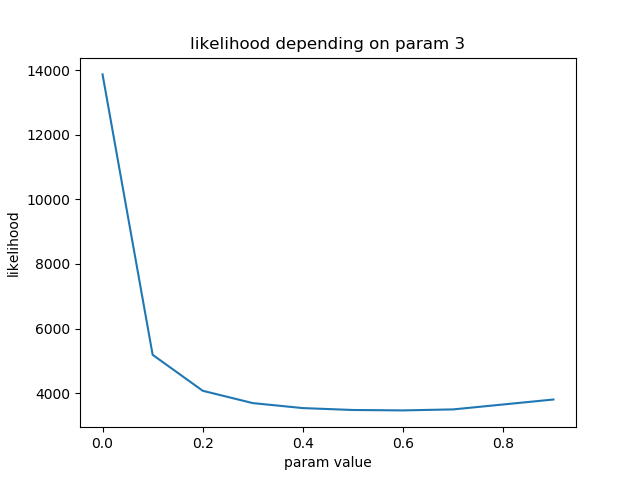
\includegraphics[scale=0.7]{../likelihoodPlot3DNMT3KO.png}
\label{rangedelta}
\caption{Negative log-likelihood depending on parameter $\delta$; the other three parameter values are fixed.}
\end{figure}

%mSat restrictions
We evaluate the likelihood function further by investigating the borders of the function. We thus compare the value of the likelihood after each parameter was set to zero and one to the present minimum. Further, during the \ac{MLE} computation, it was striking that sometimes some parameters were difficult to identify because the range where this parameter maximizes the likelihood was wide as visible in figure \ref{rangedelta}. Therefore, another approach was to fix an interval for the parameters, which may maximize the likelihood. The best results for the parameter restrictions for mSat are shown in row two and three in table \ref{DNMT1KO} and \ref{DNMT3KO}.\newline
For both methyltransferases, the likelihood is maximized by setting $\rho$ to one. $\tau$ and $\delta$ do not change significantly compared to the result without parameter restriction for DNMT3, while $\mu$ decreases by 0.217.\newline
For DNMT1 $\tau$ decreases and $\mu$ increases a bit such that all parameters besides $\delta$ are very high. Regularly, the interpretation of a high $\rho$ would be that the enzyme falls off at each \ac{bp}, but in this case, if $\tau$ is next to one too, the \ac{DNMT} will immediately bind again. In this model, the enzyme can be interpreted as very processive. We are not able to distinguish between a low disassociation probability and a very high dis- and reassociation probability as both combinations lead to the event that the methyltransferase is bound to one \ac{bp} and its successor. Thus, DNMT1 is interpreted as very processive and the result with $\rho=1$ and $\tau \approx 1$ is similar to the previous result.\newline
Another very likely scenario for DNMT3 is, if $\tau$ was set to one. Then $\rho$ is approximately one, but the methylation probabilities decrease compared to the approach without parameter restriction. The interpreting is different here, because the methylation activity is low. DNMT3 seems to work processive in this case but methylation events occur rather rarely.\newline
In the third scenario of DNMT1 and locus mSat, $\mu$ was restricted to the interval [0.8,1]. Compared to row one of table \ref{DNMT3KO}, both parameter estimations are very similar again; only the disassociation probability is even lower. Both results suggest a processive behaviour of DNMT1 with high methylation probabilities.\\

In sum by considering the mSat-locus we found that DNMT1 has a very high association probability and low disassociation probability and vice versa for DNMT3. Moreover the de novo methylation rate is lower for DNMT1 than for DNMT3, whereby the maintenance methylation rate is higher for DNMT1. Finally, we saw that the methylation rates stay low if we set $\rho$ and $\tau$ to one for DNMT1 contrary to DNMT3.

\subsection{Afp}
\label{Afp}
%DNMT1KO
The second locus considered is the alpha feto protein gene (Afp). If DNMT1 was knocked-out and no parameters were restricted, the association parameter was at its highest bound and the disassociation parameter at its lowest, where the methylation parameters both had a value of 0.8 to 0.9. This result should be excluded from further conclusions because with a association probability of zero, the enzyme will never bind and thus all other parameter are negligible.\newline
By restricting the de novo methylation rate to one, the negative log-likelihood was minimized. Hereby the disassociation probability is still close to one, but the association probability is increased. Further, $\mu$ is about 0.5. Assuming the methyltransferase binds ($\tau \neq 0$), especially the de novo methylation and disassociation probability is high, thus DNMT3 will methylate and disassociate with high probability after binding to the DNA.\newline
In a second test, both methylation probabilities were restricted to one. As a result, $\tau$ decreases slightly to 0.124, but $\rho$ does not change. The interpretation of this result can thus be seen similar to the previous one.\\

%DNMT3KO
For DNMT3a/bKO first the case without parameter restrictions is considered again. In contrast to DNMT1KO, $\rho$ and $\delta$ are close to zero, whereas the association probability with 48.8\% and the maintenance methylation probability with 36.6\% are medium high. Therefore, DNMT1 is more likely to bind, performs less methylation and disassociates less often. Moreover, DNMT1 only performs maintenance activity.\newline
The parameter restrictions which maximized the likelihood are $\mu = 1$ and $0.8 \leq \mu \leq 1$, thus a higher $\mu$ seems to be even more likely than our original \ac{MLE}-result of the Afp-locus. First, resulting from the parameter restriction $\mu = 1$, the dis- and association probability are similar at 70-80\%, while the probability of DNMT3 to transfer a methyl-group to a yet unmethylated \ac{CpG} is 0.448. Concluding, the DNA-methyltransferase binds to and falls off the DNA more often if it gets restricted to always perform maintenance methylation. Another restriction that maximized the likelihood was if $\mu$ is not exactly equal to one but lays in the interval from 0.8 to one. The parameter were estimated as 0.51($\rho$), 0.866($\tau$), 0.8($\mu$), 0.267($\delta$). Thereby we see if the methylation rates are lower, the association probability increases, while the dissociation rate decreases. Concluding, there is a relation between the methylation rate an the length of \acp{CpG}, where DNMT1 is associated: the larger the methylation rate, the smaller the association length of the \ac{DNMT}. For this locus and DNMT3a/bKO maintenance methylation parameters with higher values seem to be more probable.\\

Summarizing, we do not receive very good results for the Afp-locus without parameter restrictions as the likelihoods are significantly worse than the ones with restrictions. Further, the parameter estimation for DNMT3 is not applicable as the binding probability is zero. Including parameter restrictions, the likelihood is maximized using relatively high methylation probabilities, where $\delta$, $\mu$ or both parameters are at their maximum. Anyway, there are clear distinctions between the two methyltransferases. Where for DNMT3 either $\delta$ or $\delta$ and $\mu$ are very high, for DNMT1 $\delta$ is never high. Additionally, the de novo methyltransferase may be summarized as rare associating and frequent detaching while the maintenance methyltransferase will frequently bind and disassociate with lower probability than DNMT3 from the DNA sequence. Thus, DNMT1 works more processive than the previous-named one.

\subsection{IAP}
\label{IAP}
%DNMT1
IAPLTR1(IAP) is the final locus considered here. For this locus and DNMT1 a likelihood was retrieved that could only be slightly maximized by parameter restriction. Thus, the maximization worked very well and the results may be interpreted as very close to the optimum. These results show that DNMT1 has a very high binding affinity at this locus as the value of $\tau$ is close to one. Further, the probability to stay bound is high, which is indicated by a low disassociation probability. In general, the methylation activity of DNMT1 at IAP is similar to previous results as the maintenance methylation probability is about 0.8 and the de novo methylation probability falls into the interval 0.4 to 0.5.\newline
There were two edge cases which resulted in better likelihoods. First, the case where $\rho$ is equal to one. And second, the case where the maintenance methylation probability was restricted to its maximum value. In both cases, the four parameter, describing the methylation process of DNMT1, were very similar. The value of the association parameter is again very high with 0.901. Furthermore, the parameter suggest the enzyme will always perform maintenance methylation when bound. Only the parameter $\delta$ and $\rho$ are smaller for the restriction $\mu = 1$. With 0.375 and 0.391 the values of $\delta$ are a touch of smaller than the first mentioned estimation for this locus. What surprises is the value of $\rho$. With 0.974 and one $\rho$ is the inverse of its value without restrictions. The very high association and disassociation values lead to the assumption that DNMT1 will attach and detach multiple times while methylating. Because the probability of disassociating from the DNA is one, the enzyme detaches after each \ac{bp}. Further, because the probability to associate decreased a bit compared to the result suggesting a very processive DNMT1, it may be assumed that the enzyme is less often bound to the DNA sequence. Hence, the high maintenance methylation rate is not surprising. But, finally said, it cannot be excluded that the high rate of detachments, paired with a high number of reattachments, is caused by the model. As the binding states of an enzyme not disassociating and an enzyme dis- and reassociating are the same, we sometimes cannot distinguish the processive behaviour of an enzyme from one with many association changes.\\

%DNMT3
For DNMT3 our \ac{MLE} achieves a likelihood value of 2675. The methylation probabilities are medium high to low with 0.028 for $\mu$ and 0.566 for $\delta$. For the binding probabilities a value of zero was estimated respectively. Therefore, DNMT3 would never bind to the DNA and the methylation probabilities are invalid. We thus disregard the analysis and the result itself from further obligations.\newline
We focus on our results of DNMT3 with the binding parameters $\rho$ and $\tau$ restricted to one. The methylation parameters may be summarised as very small with $\mu$ being 0.27 and $\delta$ being around about 0.2. Also, the binding parameters are related between the two results. The binding probability is almost or exact one and the segregation probability restricted to one in the first case and 0.9 in the second case, where $\tau = 1$. Compared to the results of DNMT1KO from different loci, it is surprising that the maintenance methylation probability is higher than the de novo methylation probability. In general, the methylation probability seems to be very low, whereas there is de- and reattachment at almost every \ac{bp}. There is only one similar result in our table yet. For mSat and binding probabilities equal to one, the methylation probabilities are small, too. As mentioned earlier, a high disassociation probability, coupled with a maximal attachment rate, is equipollent to a processive working enzyme. We therefore can conclude, that a high dis- and reattachment probability and thus processivity may be possible and that it implies a low methylation rate.\\

Summarizing, the results of DNMT1 and the IAP-locus are underlying previous findings. The maintenance \ac{DNMT} works very processive with high maintenance and lower de novo methylation activity. Whereas for DNMT3, excluding one invalid result, we see a very processive enzyme with low methylation rate.

\subsection{WT}
\label{WT}
\begin{figure}[h]
\begin{center}
\begin{tabularx}{\textwidth}{l|c|c|c|c|c|c}
locus&	restrictions&	$\rho$&	$\tau$&	$\mu$&	$\delta$&	likelihood\\
\hline
mSat&	&	0.56&	0.872&	$\approx1$&	0.472&	3430\\
	&	&	0&	$\approx1$&	0.051&	0.572&	\\
\hline
Afp&	&	0.026&	0.96&	0.888&	$\approx1$&	1110\\
	&	&	0.419&	0.371&	0.797&	0.914&	\\
\hline
Afp&	$0 \leq \delta1 \leq 0.3$&	0.301&	0.895&	1&	0.18&	1077\\%**
	&	&	0.988&	0.858&	$\approx0$&	$\approx1$&	\\
\hline
Afp&	$0 \leq \delta1 \leq 0.5 \wedge 0.8 \leq \delta3 \leq 1$&	0.379&	0.915&	$\approx1$&	0.5&	1056\\
	&	&	0.268&	0.754&	$\approx0$&	0.956&	\\
\hline
IAP&	&	0.416&	0.927&	0.963&	0.749&	1838\\%*
	&	&	0.708&	0.912&	0&	0.61&	\\
\hline
IAP&	$0 \leq \delta1 \leq 0.5$&	0.17&	0.876&	0.957&	$\approx0$&	1832\\%**
	&	&	0.575&	0.879&	$\approx0$&	$\approx1$&	\\
\end{tabularx}
\end{center}
\label{WT33}
\caption{Parameter for minimal negative log-likelihoods of three loci for WT after 33 cell divisions, the first row for every locus shows the parameter for DNMT1($\rho1, \tau1, \mu1, \delta1$); the second row for DNMT3($\rho3, \tau3, \mu3, \delta3$).}
\end{figure}

\begin{figure}[h]
\begin{center}
\begin{tabularx}{\textwidth}{l|c|c|c|c|c|c}
locus&	restrictions&	$\rho$&	$\tau$&	$\mu$&	$\delta$&	likelihood\\
\hline
mSat&	&	1&	0.907&	1&	0.701&	3660\\%X
	&	&	1&	0.053&	0&	0&	\\
\hline
mSat&	$0 \leq \rho1 \leq 0.2 \wedge 0.4 \leq \rho3 \leq 1$&	0.2&	1&	0.89&	0.284&	3449\\%**
	&	$\wedge 0.5 \leq \delta3 \leq 1$&	1&	0.584&	0.286&	0.694&	\\
\hline
Afp&	&	$\approx0$&	0.916&	0.87&	$\approx0$&	3510\\
	&	&	0.971&	0.963&	0.399&	0.748&	\\
\end{tabularx}
\end{center}
\label{WT33}
\caption{Parameter for minimal negative log-likelihoods of three loci for WT after 100 cell divisions, the first row for every locus shows the parameter for DNMT1($\rho1, \tau1, \mu1, \delta1$); the second row for DNMT3($\rho3, \tau3, \mu3, \delta3$).}
\end{figure}

\section{Approximative Bayesian Computation}
\label{ABC}